\documentclass{beamer}
\usepackage[latin1]{inputenc}
\usepackage{times}
\usepackage{tikz}
\usetheme{Luebeck}
%\usecolortheme{albatross}
\usepackage{amsmath,amsfonts,amsthm,amssymb}
\usepackage{setspace}
\usepackage{Tabbing}
\usepackage{fancyhdr}
\usepackage{lastpage}
\usepackage{extramarks}
\usepackage{chngpage}
\usepackage{soul,color}
\usepackage{graphicx,float,wrapfig}
\usepackage{xcolor}
\usepackage{listings}
\usepackage{float}
%\usepackage{subfloat}
\usepackage{subfig}
\usepackage{caption}
\usepackage{enumitem}
\usepackage{algpseudocode}

\definecolor{darkorange}{RGB}{240, 120, 0}
\definecolor{darkgreen}{RGB}{0, 128, 0}

\setbeamercolor{background canvas}{bg=white}
\setbeamercolor{frametitle}{fg=white, bg=darkorange}
\setbeamercolor{normal text}{bg=black,fg=black}
\setbeamercolor{structure}{bg=black, fg=darkorange}


\lstdefinestyle{customc}{
  belowcaptionskip=1\baselineskip,
  breaklines=true,
  frame=L,
  xleftmargin=\parindent,
  language=C,
  showstringspaces=false,
  basicstyle=\footnotesize\ttfamily,
  keywordstyle=\bfseries\color{green!40!black},
  commentstyle=\itshape\color{purple!40!black},
  identifierstyle=\color{blue},
  stringstyle=\color{orange},
}

\title{Lecture 12: SVD, Procrustes Analysis}
\date{2/23/2016}
\institute{Chris Tralie, Duke University}
\author{COMPSCI/MATH 290-04}
\begin{document}

\frame{\titlepage}

\begin{frame}{Announcements}
\begin{itemize}[label=$\vartriangleright$]

\item Group Assignment 1 Full Submission Due next Tuesday 11:55 PM

\item Hackathon Saturday 2/27 4:00 PM - 10:00 PM Gross Hall 330

\item Rank Top 3 Final Project Choices By Next Wednesday 3/2

\end{itemize}

\end{frame}

\begin{frame}{Table of Contents}
\begin{itemize}[label=$\blacktriangleright$]
	\item Ray Tracing Special Case
\end{itemize}
\begin{itemize}[label=$\vartriangleright$]
	\item PCA Review
\end{itemize}
\begin{itemize}[label=$\vartriangleright$]
	\item Singular Value Decomposition
\end{itemize}
\begin{itemize}[label=$\vartriangleright$]
	\item Procrustes Distance
\end{itemize}
\begin{itemize}[label=$\vartriangleright$]
	\item Final Projects
\end{itemize}
\end{frame}

\begin{frame}{Ray Tracing Special Case}

\begin{figure}[t]
\centering
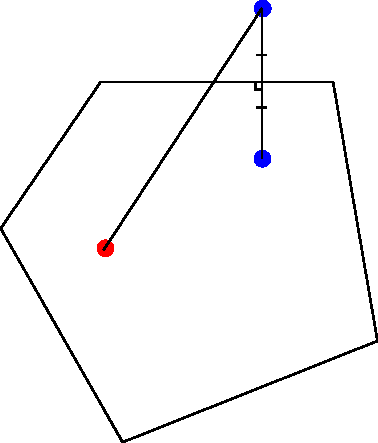
\includegraphics[width=0.5\textwidth]{ImageSourcesDrawn1.pdf}
\end{figure}

\end{frame}


\begin{frame}{Ray Tracing Special Case}

\begin{figure}[t]
\centering
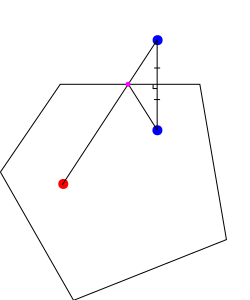
\includegraphics[width=0.5\textwidth]{ImageSourcesDrawn2.pdf}
\end{figure}

\end{frame}


\begin{frame}{Ray Tracing Special Case}

\begin{figure}[t]
\centering
\includegraphics[width=0.5\textwidth]{ImageSourcesDrawn3.pdf}
\end{figure}

\end{frame}


\begin{frame}{Ray Tracing Special Case}

\begin{figure}[t]
\centering
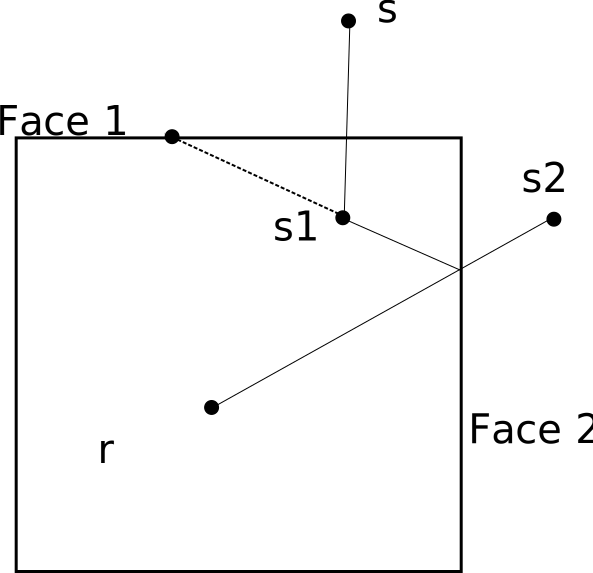
\includegraphics[width=0.5\textwidth]{SecondOrderSpecialCase.pdf}
\end{figure}

\end{frame}

\begin{frame}{Table of Contents}
\begin{itemize}[label=$\vartriangleright$]
	\item Ray Tracing Special Case
\end{itemize}
\begin{itemize}[label=$\blacktriangleright$]
	\item PCA Review
\end{itemize}
\begin{itemize}[label=$\vartriangleright$]
	\item Singular Value Decomposition
\end{itemize}
\begin{itemize}[label=$\vartriangleright$]
	\item Procrustes Distance
\end{itemize}
\begin{itemize}[label=$\vartriangleright$]
	\item Final Projects
\end{itemize}
\end{frame}

\begin{frame}{PCA Review}

Organize point cloud into $N \times d$ matrix, each point {\em along a column}

\[ X = \left[ \begin{array}{cccc} | & | & \hdots & | \\ \vec{v_1} & \vec{v_2} & \vdots & \vec{v_N} \\ | & | & \hdots & | \end{array} \right] \]

Choose a unit column vector direction $u \in \mathbb{R}^{d \times 1}$

Then 

\[ d = u^TX \]

gives projections onto $u$

\uncover<2->{
\begin{itemize}[label=$\vartriangleright$]
\item More consistent with what we've done; points in columns
\end{itemize}
}

\end{frame}

\begin{frame}{PCA New Convention}

\[ d = u^TX \]

\uncover<2->{
\begin{itemize}[label=$\vartriangleright$]
\item How to express the sum of the squares of the dot products?
\end{itemize}
}

\uncover<3->{
\[ dd^T \]
}

\uncover<4->{
\[ dd^T = (u^TX)(u^TX)^T = u^TXX^Tu \]
Want to find $u$ that maximizes the above quadratic form
}

\end{frame}

\begin{frame}{PCA New Convention}
Use eigenvectors of $A = XX^T$ to find principal directions maximizing $u^TAu$

\[\lambda_1 = 422 \]
\begin{figure}[t]
\centering
\includegraphics[width=0.7\textwidth]{2DPCADirMax.pdf}
\end{figure}


\end{frame}

\begin{frame}{PCA Review}
Use eigenvectors of $A = XX^T$ to find principal directions maximizing $u^TAu$

\[\lambda_2 = 21.6 \]
\begin{figure}[t]
\centering
\includegraphics[width=0.7\textwidth]{2DPCADirMin.pdf}
\end{figure}


\end{frame}


\begin{frame}{Table of Contents}
\begin{itemize}[label=$\vartriangleright$]
	\item Ray Tracing Special Case
\end{itemize}
\begin{itemize}[label=$\vartriangleright$]
	\item PCA Review
\end{itemize}
\begin{itemize}[label=$\blacktriangleright$]
	\item Singular Value Decomposition
\end{itemize}
\begin{itemize}[label=$\vartriangleright$]
	\item Procrustes Distance
\end{itemize}
\begin{itemize}[label=$\vartriangleright$]
	\item Final Projects
\end{itemize}
\end{frame}

\begin{frame}{Orthogonal Matrices / Rotation Review}

\[ \left[ \begin{array}{cc} \textcolor{red}{\cos(\theta)} & \textcolor{blue}{-\sin(\theta)} \\ \textcolor{red}{\sin(\theta)} & \textcolor{blue}{\cos(\theta)} \end{array}  \right] \left[ \begin{array}{c} x \\ y \end{array} \right]\]

\begin{figure}[t]
	\centering
    \includegraphics[width=0.6\textwidth]{ColumnVectorRot2.pdf}
\end{figure}

\end{frame}


\begin{frame}{Orthogonal Matrices / Rotation Review}

Inverse rotation: dot product interpretation

\[ \left[ \begin{array}{cc} \cos(\theta) & \sin(\theta) \\ -\sin(\theta) & \cos(\theta) \end{array}  \right] \left[ \begin{array}{c} x \\ y \end{array} \right]\]

\begin{figure}[t]
	\centering
    \includegraphics[width=0.6\textwidth]{ColumnVectorRotDual.pdf}
\end{figure}

\end{frame}



\begin{frame}{Orthogonal Matrices / Rotation Review}

In general

\[ R = \left[ \begin{array}{cccc} | & | & \vdots & | \\ \vec{u_1} & \vec{u_2} & \hdots & \vec{u_N} \\ | & | & \vdots & | \end{array} \right] \]

\[\vec{u_i} \cdot \vec{u_j} = 1, i = j \]
\[\vec{u_i} \cdot \vec{u_j} = 0, i \neq j \]

In 3D, 

\[ \vec{u_1} \times \vec{u_2} = \vec{u_3} \]

for a pure rotation

\end{frame}



\begin{frame}{Orthogonal Matrices / Rotation Review}

\[ R = \left[ \begin{array}{cccc} | & | & \vdots & | \\ \vec{u_1} & \vec{u_2} & \hdots & \vec{u_N} \\ | & | & \vdots & | \end{array} \right] \]

\[ R^T = \left[ \begin{array}{ccc} - & \vec{u_1} & - \\ - & \vec{u_2} & - \\ \hdots & \vdots & \hdots \\ - & \vec{u_N} & - \end{array} \right] \]

\[\vec{u_i} \cdot \vec{u_j} = 1, i = j \]
\[\vec{u_i} \cdot \vec{u_j} = 0, i \neq j \]

\[R^TR = RR^T = I \]

\end{frame}

\begin{frame}{Singular Value Decomposition}

Given an $m \times n$ matrix $A$, the SVD of $A$ is

\[ A = U S V^T \]

\begin{itemize}[label=$\vartriangleright$]
\item
$U$ is an $M \times M$ rotation matrix

\item
$S$ is an $M \times N$ matrix, where $S_{ij} = 0$ $i \neq j$

\item
$V$ is an $N \times N$ rotation matrix

\end{itemize}


\[ A =  \left[ \begin{array}{cccc} | & | & \vdots & | \\ \vec{u_1} & \vec{u_2} & \hdots & \vec{u_M} \\ | & | & \vdots & | \end{array} \right]  \left[  \begin{array}{ccccc} s_1 & 0 & 0 & \hdots & 0 \\ 0 & s_2 & 0 & \hdots & 0 \\ 0 & 0 & s_3 & \hdots & 0 \\ \hdots & \vdots & \vdots & \hdots & \vdots \\ 0 & 0 & \hdots & s_M & \hdots 0  \end{array} \right] \left[ \begin{array}{ccc} - & \vec{v_1} & - \\ - & \vec{v_2} & - \\ \hdots & \vdots & \hdots \\ - & \vec{v_N} & - \end{array} \right] \]

\end{frame}


\begin{frame}{Singular Value Decomposition}

\[ A = U S V^T \]


\[ A =  \left[ \begin{array}{cccc} | & | & \vdots & | \\ \vec{u_1} & \vec{u_2} & \hdots & \vec{u_M} \\ | & | & \vdots & | \end{array} \right]  \left[  \begin{array}{ccccc} s_1 & 0 & 0 & \hdots & 0 \\ 0 & s_2 & 0 & \hdots & 0 \\ 0 & 0 & s_3 & \hdots & 0 \\ \hdots & \vdots & \vdots & \hdots & \vdots \\ 0 & 0 & \hdots & s_M & \hdots 0  \end{array} \right] \left[ \begin{array}{ccc} - & \vec{v_1} & - \\ - & \vec{v_2} & - \\ \hdots & \vdots & \hdots \\ - & \vec{v_N} & - \end{array} \right] \]

\begin{itemize}[label=$\vartriangleright$]

\uncover<2->{
\item $s_1 > s_2 > s_3 > ... > s_M$
}

\uncover<3->{
\item $U$ holds the eigenvectors of $AA^T$
}

\uncover<4->{
\item $V$ holds the eigenvectors of $A^TA$
}

\uncover<5->{
\item Each $s$ is the square root of corresponding eigenvalue of $AA^T$ and $A^TA$
(they're the same!)
}

\end{itemize}

\end{frame}


\begin{frame}{Singular Value Decomposition: Example}

\begin{figure}[t]
	\centering
    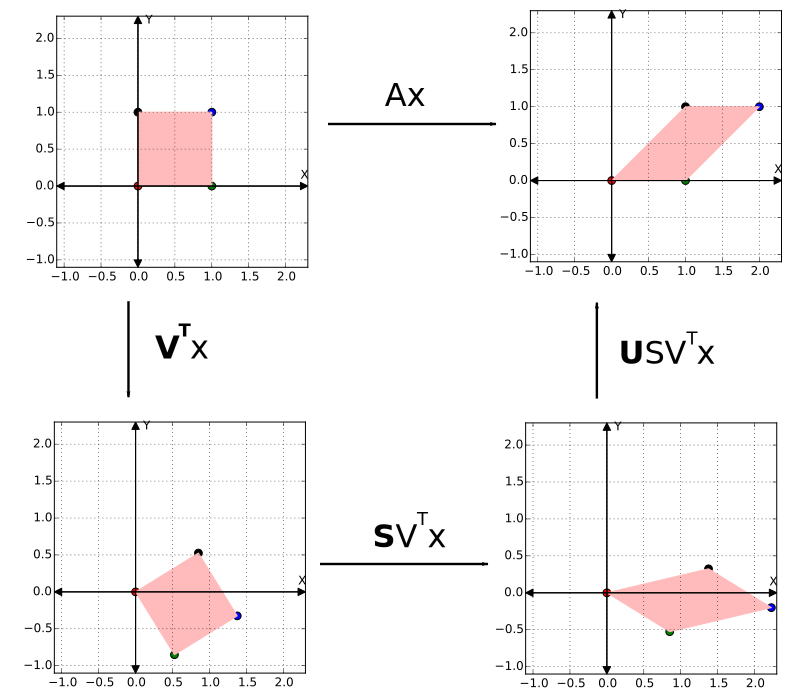
\includegraphics[width=0.8\textwidth]{2DShear.pdf}
\end{figure}


\end{frame}


\begin{frame}{Singular Value Decomposition: Example}

\begin{figure}[t]
	\centering
    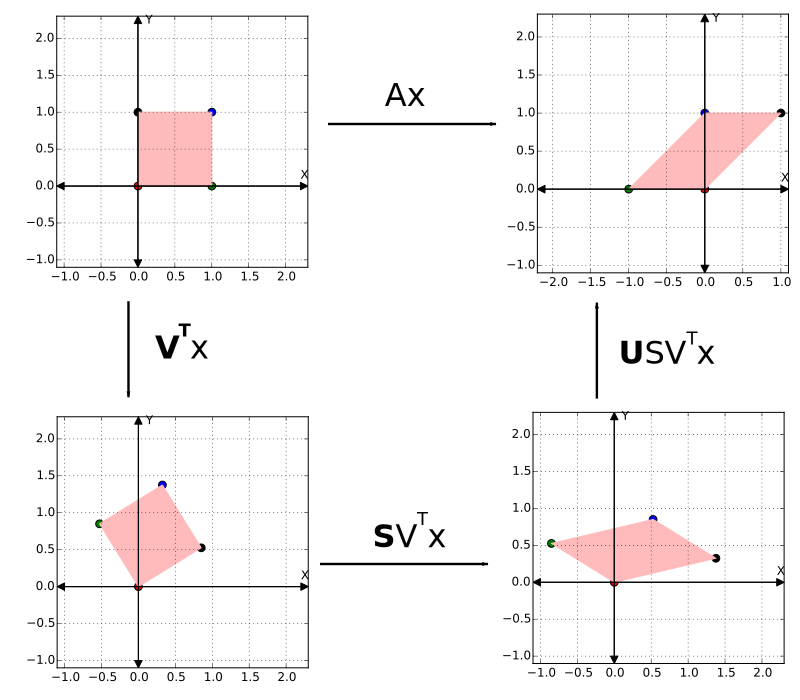
\includegraphics[width=0.8\textwidth]{2DFlipSkewAll.pdf}
\end{figure}


\end{frame}


\begin{frame}{Singular Value Decomposition: Example}

\begin{figure}[t]
	\centering
    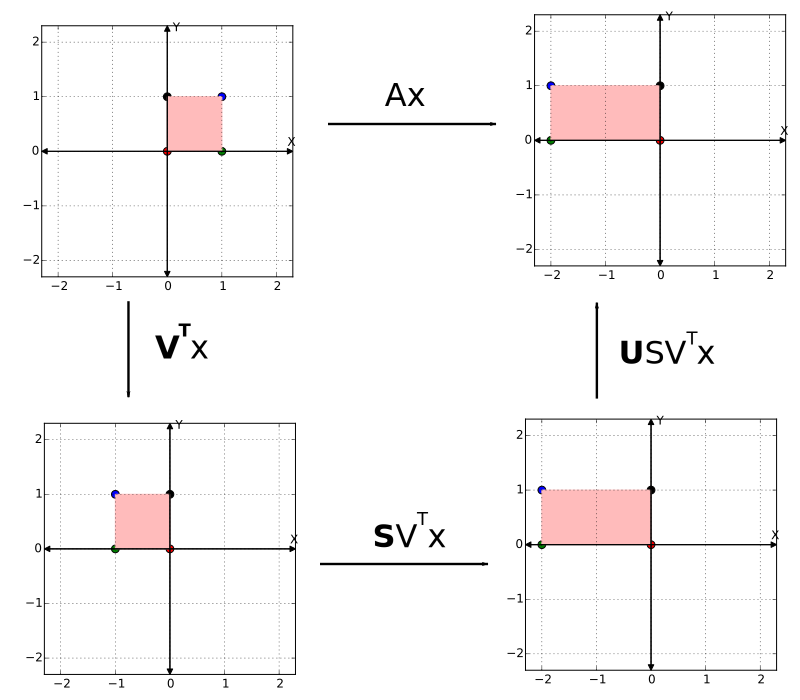
\includegraphics[width=0.8\textwidth]{2DScaleAll.pdf}
\end{figure}


\end{frame}

\begin{frame}{Singular Value Decomposition $\rightarrow$ PCA}

\[ A = U S V^T \]



\begin{itemize}[label=$\vartriangleright$]

\item $s_1 > s_2 > s_3 > ... > s_M$

\item $U$ holds the eigenvectors of $AA^T$

\item $V$ holds the eigenvectors of $A^TA$

\item Each $s$ is the square root of corresponding eigenvalue of $AA^T$ and $A^TA$

\end{itemize}

Let $X$ be a $3 \times N$ matrix of points along columns.

Can we use SVD($X$) to do PCA?

\end{frame}


\begin{frame}{Singular Value Decomposition $\rightarrow$ PCA}

\[ X = U S V^T \]

\begin{itemize}[label=$\vartriangleright$]

\item Columns of $U$ give principal components

\item Squares of corresponding $S$ gives sum of squared magnitudes along directions of $U$

\item Coordinates along $U$ directions?

\end{itemize}

\end{frame}


\begin{frame}{Table of Contents}
\begin{itemize}[label=$\vartriangleright$]
	\item Ray Tracing Special Case
\end{itemize}
\begin{itemize}[label=$\vartriangleright$]
	\item PCA Review
\end{itemize}
\begin{itemize}[label=$\vartriangleright$]
	\item Singular Value Decomposition
\end{itemize}
\begin{itemize}[label=$\blacktriangleright$]
	\item Procrustes Distance
\end{itemize}
\begin{itemize}[label=$\vartriangleright$]
	\item Final Projects
\end{itemize}
\end{frame}


\begin{frame}{Procrustes Distance}

\begin{figure}[t]
	\centering
    \includegraphics[width=0.6\textwidth]{procrustes.png}
\end{figure}

\url{http://www.procrustes.nl/gif/illustr.gif}

\end{frame}

\begin{frame}{Procrustes Alignment}

\begin{figure}[t]
	\centering
    \includegraphics[width=\textwidth]{ProcrustesEx1.png}
\end{figure}

\end{frame}


\begin{frame}{Procrustes Distance}

Given two point clouds $\{\vec{x_i}\}_{i=1}^N$ and $\{\vec{y_i}\}_{i=1}^N$

where $x_i$ and $y_i$ are in correspondence

Seek to minimize

\[ \sum_{i=1}^N ||R(\vec{x_i} + \vec{t}) - \vec{y_i}||_2^2 \]

over all orthogonal matrices $R$ and translation vectors $t$.  $||.||^2_2$ is squared distance

\end{frame}


\begin{frame}{Translation}
\[ \sum_{i=1}^N ||R(\vec{x_i} + \vec{t}) - \vec{y_i}||_2^2 \]

Translation is easy! Align centroids


\[ \vec{t} = \frac{1}{N} \left(\sum_{i=1}^N \vec{y_i} - \sum_{i=1}^N \vec{x_i} \right) \]

\begin{figure}[t]
	\centering
    \includegraphics[width=0.5\textwidth]{ProcrustesEx1Translated.png}
\end{figure}


\end{frame}


\begin{frame}{Rotating to Align Points: Dot Product Perspective}

\[ \vec{x_1} \cdot \vec{y_1} = ||\vec{x_1}|| ||\vec{y_1}|| \cos(\theta_1) \]

\begin{figure}[t]
	\centering
    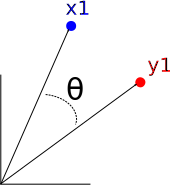
\includegraphics[width=0.4\textwidth]{PointsAlign.pdf}
\end{figure}

\end{frame}


\begin{frame}{Rotating to Align Points: Dot Product Perspective}

\[ \vec{x_1} \cdot \vec{y_1} + \vec{x_2} \cdot \vec{y_2} = ||\vec{x_1}|| ||\vec{y_1}|| \cos(\theta_1) + ||\vec{x_2}|| ||\vec{y_2}|| \cos(\theta_2) \]

\begin{figure}[t]
	\centering
    \includegraphics[width=0.5\textwidth]{PointsAlign2.pdf}
\end{figure}

\end{frame}

\begin{frame}{Rotating to Align Points: Dot Product Perspective}

\[ \vec{x_1} \cdot \vec{y_1} + \vec{x_2} \cdot \vec{y_2} = ||\vec{x_1}|| ||\vec{y_1}|| \cos(\theta_1) + ||\vec{x_2}|| ||\vec{y_2}|| \cos(\theta_2) \]

\begin{figure}[t]
	\centering
    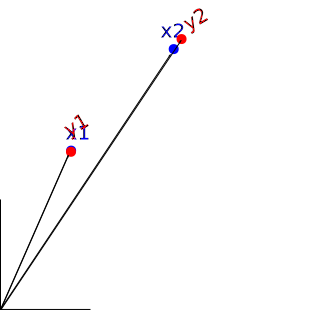
\includegraphics[width=0.3\textwidth]{PointsAlign2Rot.pdf}
\end{figure}

\uncover<2->{
\begin{itemize}[label=$\vartriangleright$]
\item Why should points further away from origin get more weight?
\end{itemize}
}

\end{frame}


\begin{frame}{Rotating to Align Points: Dot Product Perspective}

In general, how to maximize?

\[ \sum_{i = 1}^N \textcolor{blue}{R_x \vec{x_i}} \cdot \textcolor{red}{R_y \vec{y_i}} \]
\begin{figure}[t]
	\centering
    \includegraphics[width=0.5\textwidth]{2DProcrustes1.pdf}
\end{figure}


\end{frame}


\begin{frame}{Rotating to Align Points: Dot Product Perspective}

In general, how to maximize?

\[ \sum_{i = 1}^N \textcolor{blue}{R_x \vec{x_i}} \cdot \textcolor{red}{R_y \vec{y_i}} \]

VIDEO EXAMPLE


\end{frame}

\begin{frame}{Maximizing Dot Product: First Component}

Choose first row of $R_x$, which is a projection of blue points.  Call this row $a_1$ (write as a row vector)

\[ a_1X \]

\begin{figure}[t]
	\centering
    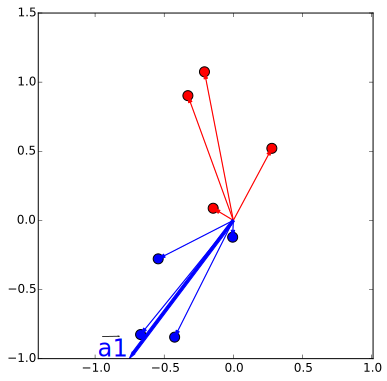
\includegraphics[width=0.5\textwidth]{2DProcrustesProj1.pdf}
\end{figure}


\end{frame}


\begin{frame}{Maximizing Dot Product: First Component}

Choose first row of $Ry$, which is a projection of red points.  Call this row $b_1$ (write as row vector)

\[ b_1 Y \]

\begin{figure}[t]
	\centering
    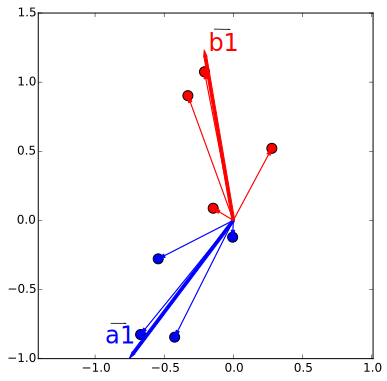
\includegraphics[width=0.5\textwidth]{2DProcrustesProj2.pdf}
\end{figure}


\end{frame}


\begin{frame}{Maximizing Dot Product: First Component}

\[a_1 X, b_1 Y \]

How to write $\sum_{i=1}^N (\vec{a_1} \cdot \vec{x_i})(\vec{b_1} \cdot \vec{y_i})$ in matrix form?

\uncover<2->{
\[  (a_1 X) (b_1 Y)^T = a_1 X Y^T b_1^T \]
}

\begin{figure}[t]
	\centering
    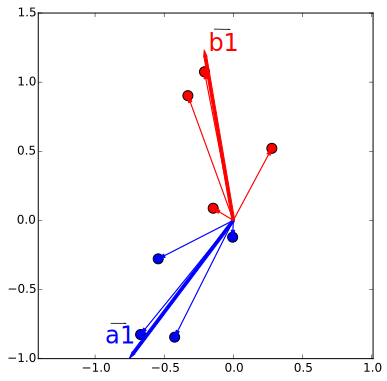
\includegraphics[width=0.4\textwidth]{2DProcrustesProj2.pdf}
\end{figure}


\end{frame}


\begin{frame}{Maximizing Dot Product: First Component}

How to find $u_1$ and $v_1$ that maximize this product?

\[  (a_1 X) (b_1 Y)^T = a_1 X Y^T b_1^T \]

Take SVD: $XY^T = USV^T$ and substitute in

\[ a_1 U S V^T b_1^T \]


\end{frame}

\begin{frame}

Continued next time...

\end{frame}

\end{document}

